\section{Experiments}
\label{sec:experiment}
% \subsection{Experimental Setup} 
\subsection{Datasets}
\textbf{Synthetic}\quad Inspired by \citet{kossen2022active}, we construct a synthetic dataset of $N=8,000$ samples with $L=10$ non-i.i.d. timepoints. Each timepoint contains two features: \textit{digit} and \textit{counter}. Labels are the cumulative sum of the digits, when the counter values are zero. We elaborate below.

% a sequence of \textit{digit} features that are summed at locations where \textit{counter} feature indicates (with a zero value). That is, the output labels are comprised of the cumulative sum of the counter-indicated digits. We expound below.


The \textit{digit} feature is a sequence of uniformly random $L$ integers from $\{0, 1, 2\}$, e.g., $1010220110$. The \textit{counter} feature is created by concatenating countdown sequences that begin with randomly chosen starting values from $\{0, 1, 2\}$ and truncating to a fixed length of $L$. For example, starting values $2$, $1$, $2$, and $1$ yield $210$, $10$, $210$, $10$, and the final counter feature is their concatenation $2101021010$ (of length $L$). Unlike \citet{kossen2022active}, we assign labels at every timestep: 
% $y_t$ is the cumulative sum of the digit values up to time $t$ (inclusive) where the corresponding counter value is $0$, i.e.,
$y_t=\sum_{t'=1}^{t}\mathrm{digit}_{t'}\mathbb{I}\{\mathrm{counter}_{t'}=0\}$; for example, label $0011333444$ in the case of $\genfrac{}{}{0pt}{}{\mathrm{counter:}}{\mathrm{digit:}}  
 \genfrac{}{}{0pt}{}{21\underline{0}1\underline{0}21\underline{0}1\underline{0}}{10\mathbf{1}0\mathbf{2}20\mathbf{1}1\mathbf{0}}$. The policy should begin with acquiring the digit and counter at 
$t=1$, then acquiring the digit at the next anticipated timestep where $\mathrm{counter}=0$, then acquiring the \textit{counter} again to locate the next $\mathrm{counter}=0$ timestep, and repeat. Following \citet{kossen2022active}, we split data into train/val/test ($70\%/15\%/15\%$).

\textbf{ADNI}\quad The Alzheimer's Disease Neuroimaging Initiative (ADNI) dataset\footnote{\url{https://adni.loni.usc.edu}}~\citep{petersen2010alzheimer} is a longitudinal, multi-center, observational study. Patients are categorized into cognitively unimpaired, mild cognitive impairment, and Alzheimer's Disease \citep{o2008staging, o2010validation}. Following~\citet{qin2024risk}, we use $N=1,002$ patients with four biomarkers extracted from PET (FDG and AV45) and MRI (Hippocampus and Entorhinal) across $L=12$ visits, and split the dataset into train/val/test ($64\%/16\%/20\%$). \looseness-1
% Each patient may have a different pattern of missing features or labels, and we only report the results based on those that have a diagnosis label. %Appendix $\ref{sec:cost}$ provides further details.

\textbf{OAI}\quad The Osteoarthritis Initiative (OAI) dataset\footnote{\url{https://nda.nih.gov/oai/}} contains $N=4,796$ patients (left/right knees) monitored up to $96$ months. We use the tabular data from~\citet{chen2024unified} and joint space width, totaling $27$ features per visit across $L=7$ visits. We predict the two clinical scores: Kellgren-Lawrence grade (KLG)~\citep{kellgren1957radiological} (range $0 \sim 4$) and WOMAC pain score~\citep{mcconnell2001western} (range $0 \sim 20$). Following previous works~\citep{chen2024unified,nguyen2024active}, we merge KLG $=0$ and $1$, and define WOMAC $<5$ as no pain and $\geq 5$ as pain, and split the dataset into train/val/test ($50\%/12.5\%/37.5\%$). 

\subsection{Baselines} 
\emph{We \uline{expand the comparisons} performed in recent work} by \citet{qin2024risk} in longitudinal AFA  by comparing to \emph{two other state-of-the-art AFA methods}, {DIME}~\citep{gadgil2023estimating} and {DiFA} \citep{ghosh2023difa}, in addition to the RL method considered by \citet{qin2024risk}.
\begin{figure*}[t] 
  \centering
  % ----- 1st column -------------------------------------------------
  \resizebox{0.85\textwidth}{!}{
  \begin{subfigure}[t]{.24\textwidth}
    \centering
    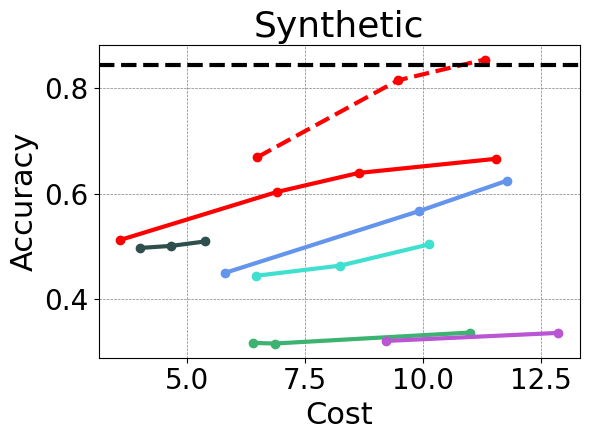
\includegraphics[width=\linewidth]{figures/synthetic.png}
    % \caption{Synthetic}\label{fig:sub1}
  \end{subfigure}
  % ----- 2nd column -------------------------------------------------
  \begin{subfigure}[t]{.24\textwidth}
    \centering
    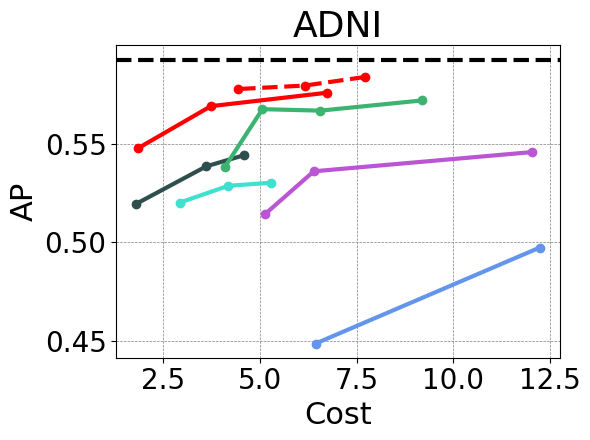
\includegraphics[width=\linewidth]{figures/adni.png}
    % \caption{ADNI}\label{fig:sub2}
  \end{subfigure}
  % ----- 3rd column -------------------------------------------------
  \begin{subfigure}[t]{.24\textwidth}
    \centering
    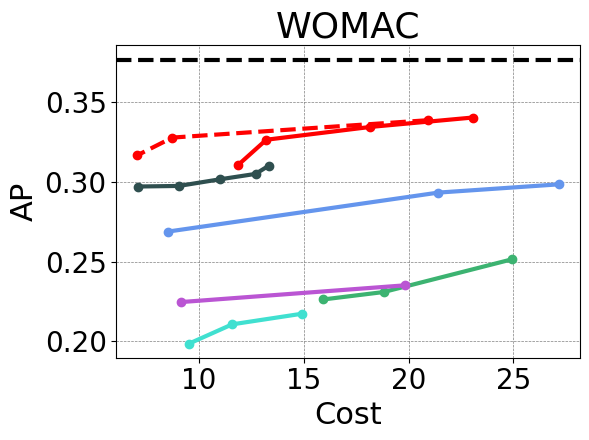
\includegraphics[width=\linewidth]{figures/womac.png}
    % \caption{WOMAC}\label{fig:sub3}
  \end{subfigure}
  % ----- 4th column -------------------------------------------------
  \begin{subfigure}[t]{.24\textwidth}
    \centering
    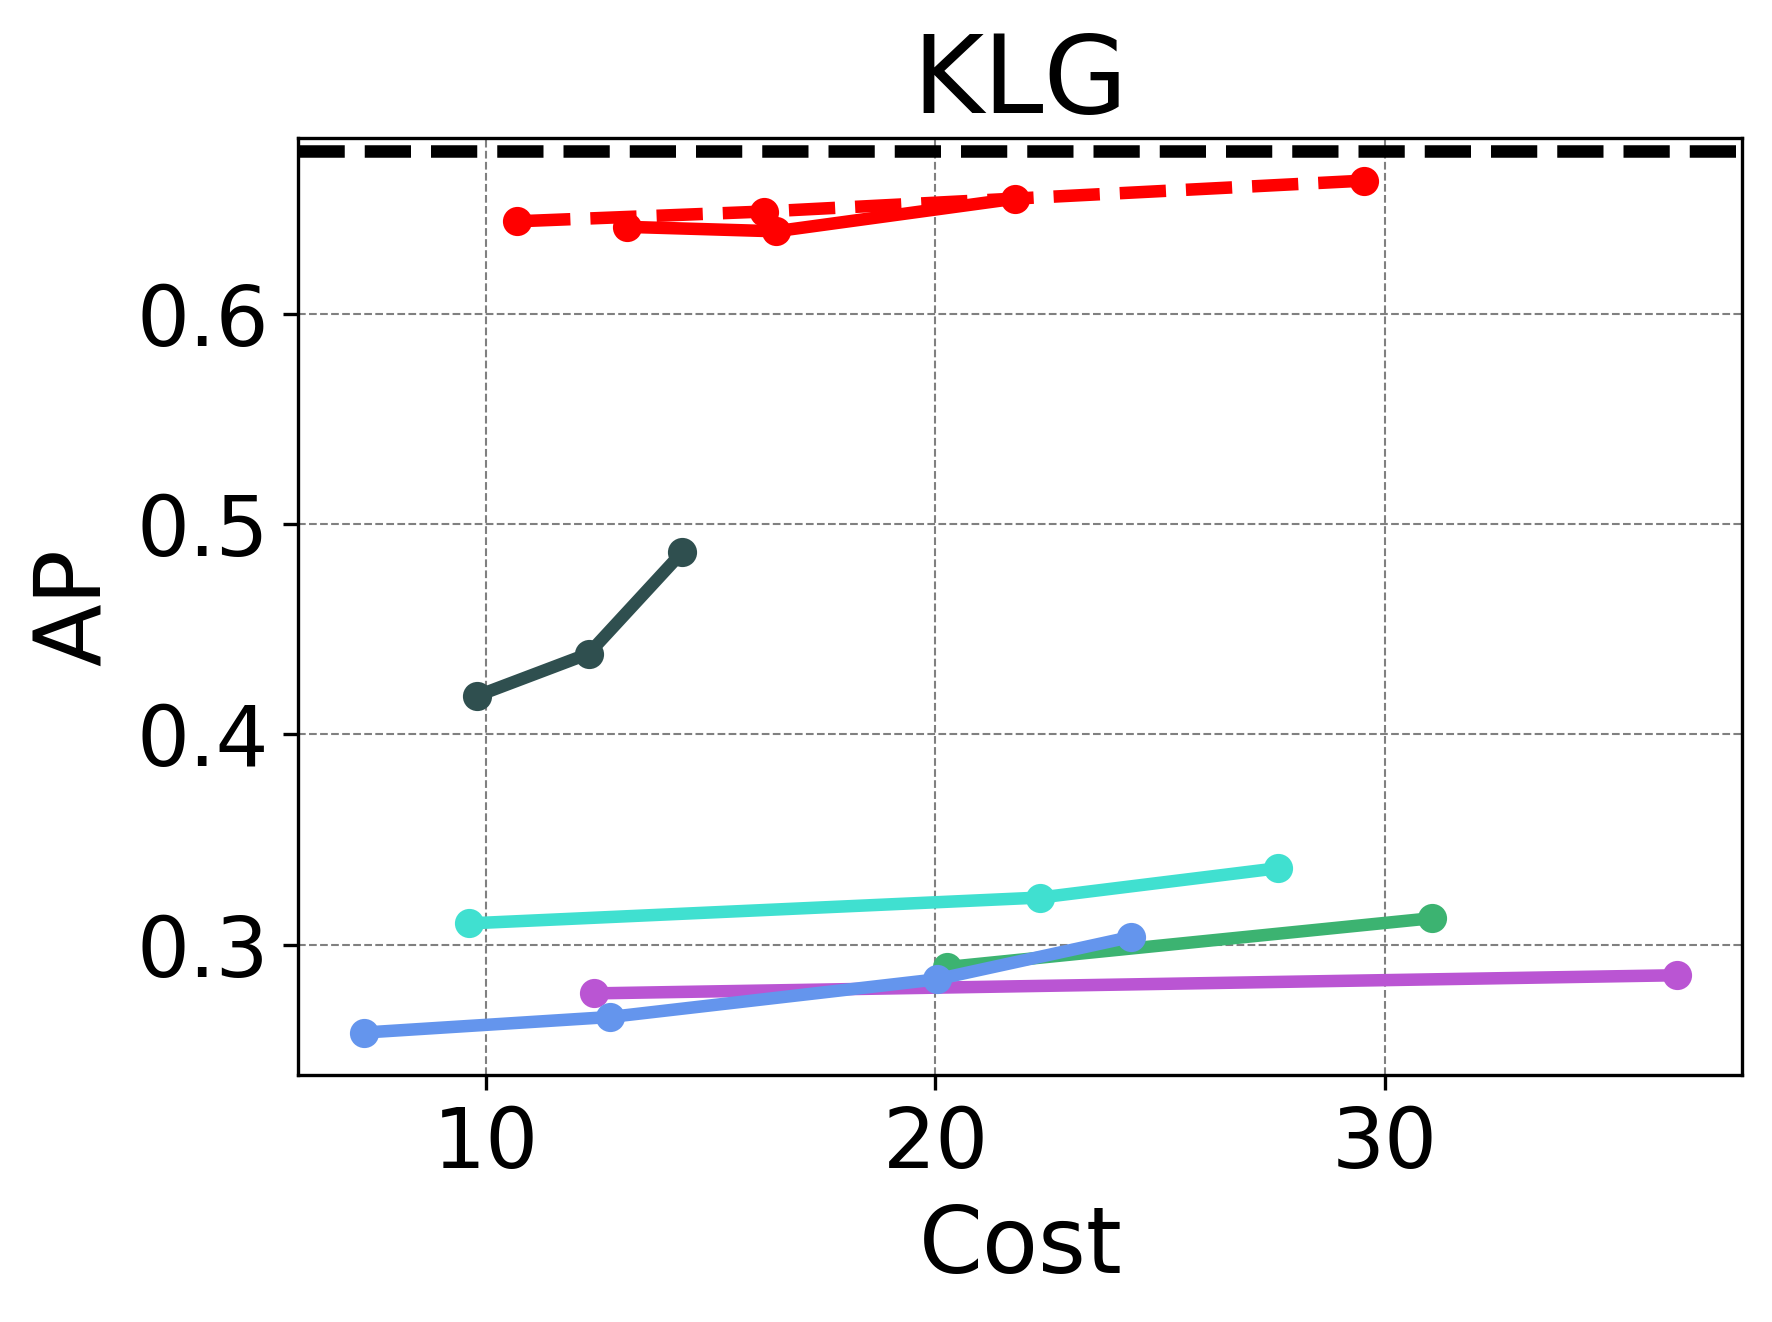
\includegraphics[width=\linewidth]{figures/klg.png}
    % \caption{KLG}\label{fig:sub4}
  \end{subfigure}
  }
  
  % \par\bigskip            % vertical gap between plots and legend
  \vspace{-0.5em}
  \begin{minipage}{\textwidth}
    \centering
    % trim=⟨left bottom right top⟩ clip    — remove surrounding whitespace if needed
    
\includegraphics[width=0.8\textwidth,trim=0 0 0 0,clip]{figures/legend_only.png}
  \end{minipage}
  \vspace{-1em}
  \caption{Performance/cost of  models 
  % on the four benchmarks 
  across various average acquisition costs (budgets). Following~\cite{kossen2022active}, we show accuracy rather than average precision for the synthetic dataset. Our NOCT estimators show the highest accuracy for a given cost. }
  \label{fig:performance}
\end{figure*}

In total, we consider the following baselines: 1) \textbf{ASAC}~\citep{yoon2019asac}: an actor-critic method to jointly train a feature selector and a predictor network; 2) \textbf{RAS}~\citep{qin2024risk}: an RL approach to decide when and which features to capture for longitudinal data where the predicted acquisition times are continuous and not restricted to certain discrete timepoints; 3) \textbf{AS} \citep{qin2024risk}: RAS with a constant acquisition interval; 4) \textbf{DIME}~\citep{gadgil2023estimating}: a greedy method to sequentially select the most informative features; 5) \textbf{DiFA} \citep{ghosh2023difa}: a Gumbel-softmax-based differentiable policy. For each baseline, \emph{we perform a comparable hyperparameter search on the validation set using the authors' original code}, and report test performance under the selected configuration. We also verify reproduction of reported results (e.g., RAS on ADNI); full details are provided in Appx.~\ref{sec:baseline}.


We adapt DIME and DiFA for longitudinal data by restricting acquisitions to either the current or future time points. Note that DIME and DiFA acquire features one at a time, allowing repeated selection within the same time step $t$, while \texttt{\OurMethod} and other baselines simultaneously select all desired features at $t$ before moving to the next time steps. An advantage of DiFA and DIME is that they can acquire more tests now or move to the next visit. \looseness-1


\subsection{Implementation}
\label{sec:implementation}

\textbf{Data Availability and Missingness.} Unlike standard AFA methods that assume fully observed data \citep{rahbar2025survey, shim2018joint, nan2015feature}, our work is general and handles missingness completely at random. This is done by excluding missing features from candidate sets and pretraining the prediction network $\hat{y}_k$, estimator $f_\theta$, and embedding network $g_\phi$ with random input-feature dropout.  


\textbf{Prediction Network Implementation.}  At each time $t$, the prediction network predicts outcomes at future timepoints $\hat{y}_k$, $k \geq t$. We train an MLP that takes all the features observed up to time t, denoted $x_{o_{1:t}}$ \footnote{$x_o$ may contain missingness inherent to the data collection process. Additionally, unobserved features (missing or not acquired) are being masked out during implementation.} and the future time indicator $k$. 
% We then define the prediction network loss as: 
% the prediction network $\hat{y}_k$ uses all features that have been observed up to $t$ (e.g., ${x}_{o_{1:t}}$), combining with future time indicator $k$. That is, we train an MLP that takes $x_{o_{1:t}}$ \footnote{$x_o$ may include missingness due to the inherent noise in data collection. Additionally, unobserved features (missing or not acquired) are being masked out during implementation.} and time indicator $k$ as its input, and apply cross-entropy loss as:
% \begin{equation}
%     \mathcal{L}_{\mathrm{pred}} = \frac{1}{L}\sum_{k=1}^{L}{\mathrm{CE}\bigl(\hat{y}_k({x}_{o_{1:t}}), y_{k}\bigr)}.
% \end{equation}
For predictions at $k > t$, the network must predict without access to any additional features beyond those observed by time $t$ (i.e., $\hat{y}_{k}(x_{o_{1:t}})$ for $k > t$). 


% To mimic the AFA process, the prediction network should be able to predict with any subset of the input features, and hence, we pre-train the prediction network with a random dropout of the input features, whose data are set to $0$. 

\textbf{\texttt{NOCT-Contrastive} Implementation.}\quad
We train the MLP predictor $\hat{y}_k$ and then train the MLP embedding network $g_\phi$. We set $\beta=\gamma=1$, $K=5$, and embedding dimension $E=32$ (Synthetic/ADNI) and $E=64$ (OAI).%, and sample $|\widetilde{\mathcal{V}}|=1000$ subsets.


\textbf{\texttt{NOCT-Amortized} Implementation.}\quad We first train the MLP predictor $\hat{y}_k$, followed by jointly fine-tuning the predictor and the MLP-based NOCT estimator $f_{\theta}$ (Eq.~\ref{eq:value_mse}) using $\lambda=1$.% Both steps use Adam~\citep{kingma2014adam} with a learning rate of $1e-3$ and use $\lambda=1$. We randomly sample $|\widetilde{\mathcal{V}}|=1000$ candidate subsets.

\textbf{Optimizer and Inference}\quad We utilize Adam~\citep{kingma2014adam} with a learning rate of $10^{-3}$. At each inference step, we evaluate a subset of 1,000 plans from the 
candidate space (see Appx. \ref{appendex:sensitivity} for a stability analysis).
% we consider a subset of $1000$   candidate plans

% \textbf{Subset Size $|\mathcal{O}|$.} For experiments, we uniformly sample $1000$ candidate acquisitions to balance effectiveness and overhead. As shown in Appx. $\ref{appendex:sensitivity}$, accuracy stabilizes and returns diminish beyond this cardinality. In practice, we observed uniform sampling is effective and fast, but other discrete optimization methods can be utilized \citep{parker2014discrete, rajeev1992discrete}.

% Following the conventional setup for longitudinal AFA tasks \citep{yoon2019asac, qin2024risk}, we consider each modality as a single feature. 
We report predictive performance results as the mean over five independent runs (standard errors for each run are provided in Appx.~\ref{appendex:results}). Feature costs and further details on the experimental setup can be found in Appx.~\ref{appendex:experiment_setup}. Moreover, Appx.~\ref{appendex:sensitivity} shows a hyperparameter sensitivity analysis, demonstrating that 
\textit{our method remains robust across different settings and can be applied without extensive tuning}.
Upon publication, we will make our code publicly available.


\subsection{Performance-Cost Results}


Fig.~\ref{fig:performance} shows results across different datasets. For each figure, the x-axis represents different average acquisition costs per instance, and the y-axis represents the performance. As the budget increases, more features can be acquired, and prediction performance typically improves. 
We varied hyperparameters to obtain prediction results under different average acquisition costs. Details on the performance-cost tradeoff hyperparameters for each method are in Appx. \ref{appendex:experiment_setup}.
% To obtain points at different average acquisition costs: (1) for RAS, AS, ASAC, and \texttt{\OurMethod‑NP} we sweep the performance-cost tradeoff hyperparameter, (2) DIME and DiFA impose budget limits, and (3) \texttt{\OurMethod‑P} uses both the performance-cost tradeoff hyperparameter and the budget limits. For further details about the trade-off parameter in Appendix \ref{appendex:experiment_setup}.

\textbf{Synthetic Dataset.} Following~\citet{kossen2022active}, we use accuracy for performance on the synthetic dataset. The \texttt{NOCT-Contrastive} estimator outperforms the baselines, followed by the  \texttt{NOCT-Amortized} estimator, suggesting that the baseline methods may not adequately model dependencies between features and necessary acquisitions. 


\textbf{ADNI Dataset.} Following \citet{qin2024risk}, we show the average precision (AP) result for different costs. Both estimator variants of \texttt{\OurMethod} consistently outperform all other baseline methods while using lower overall acquisition cost.
% RAS~\citep{qin2024risk} and DIME~\citep{gadgil2023estimating} also appear to be strong baselines, as they both allows dynamic selection in when and which features to select. AS turned out to be less effective without being able to adapt to the acquisition interval, and ASAC~\citep{yoon2019asac} \todo{add why ASAC not so good}

% \begin{figure*}[!ht]
%   \centering
%   % Left column
%   \begin{minipage}[t]{0.49\textwidth}
%     \centering
%     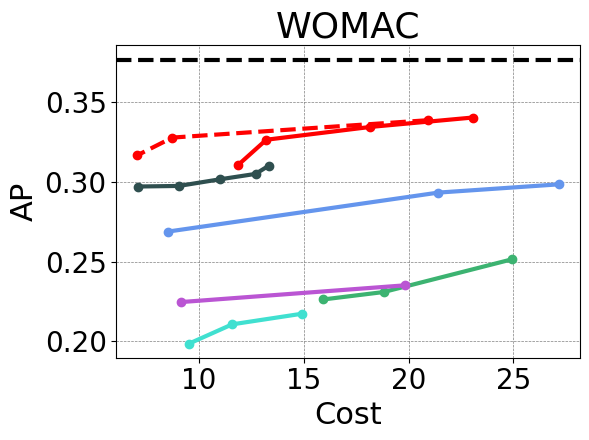
\includegraphics[width=\linewidth]{figures/womac.png}
%     \captionsetup{skip=2pt}
%     \captionof{figure}{AP and ROC vs. average cost on WOMAC prediction}
%     \label{fig:womac}
%   \end{minipage}\hfill
%   \begin{minipage}[t]{0.49\textwidth}
%     \centering
%     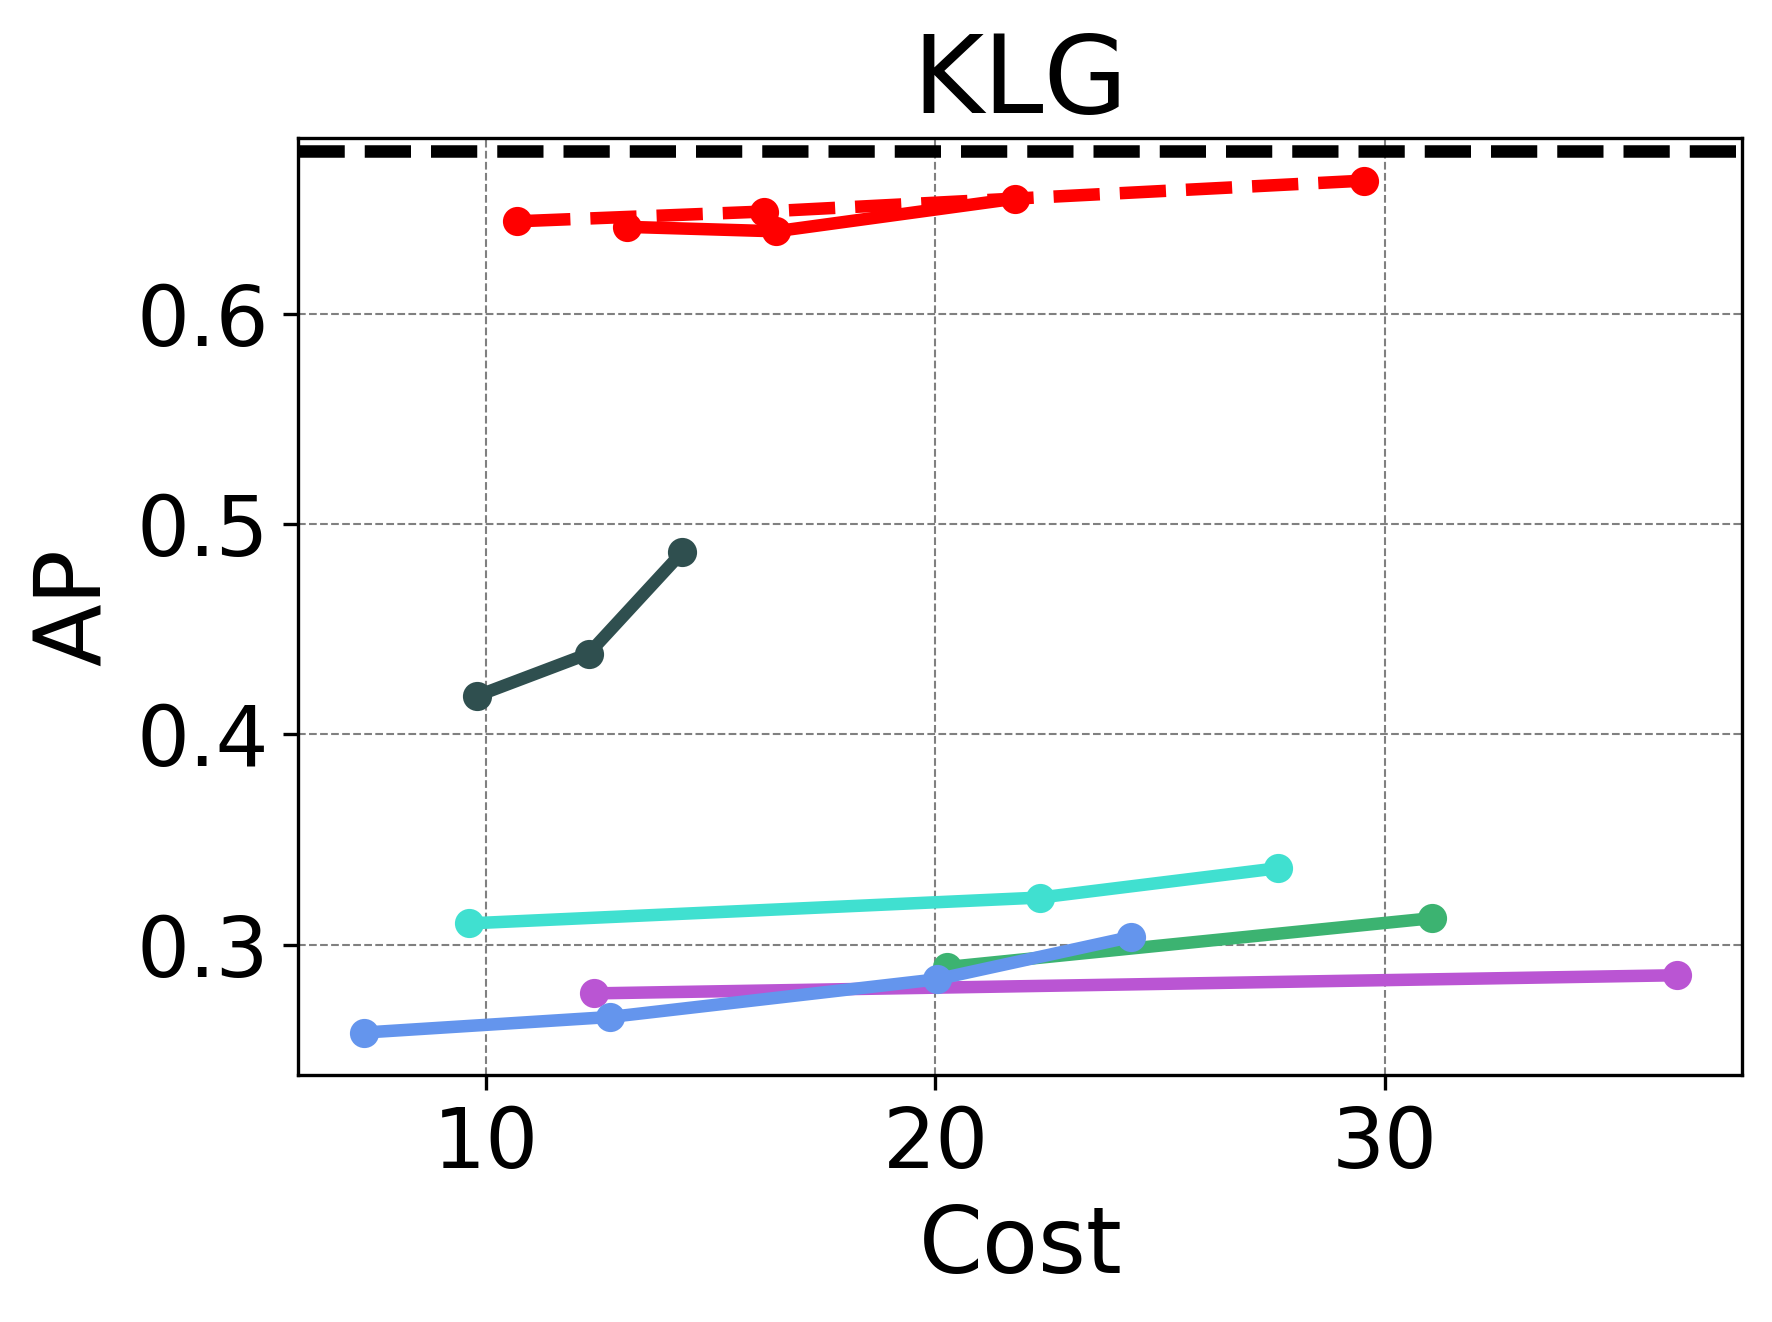
\includegraphics[width=\linewidth]{figures/klg.png}
%     \captionsetup{skip=2pt}
%     \captionof{figure}{AP and ROC vs. averagecost on KLG prediction}
%     \label{fig:klg}
%   \end{minipage}
% \end{figure*}
\textbf{OAI Dataset.} We report AP on KLG and WOMAC prediction (Fig.~\ref{fig:performance}). The \texttt{\OurMethod} again outperforms the baselines, while RL-based approaches (ASAC, AS, and RAS) underperform compared to the greedy approach (DIME), suggesting that RL-based frameworks may struggle with the complexity and noise of longitudinal feature acquisition. 
\begin{table*}[ht]
\captionsetup{skip=2pt}
\caption{Result comparisons of using the feature values, $\hat{y}$ prediction embedding (last hidden layer), and learned representation $g_\phi(\cdot)$ to gather instances for \texttt{NOCT-Contrastive} inference. We report the mean $\pm$ standard errors across five runs.}
\label{tab:embedding}
% \vspace{-0.1in}
\begin{center}
\begin{sc}
\resizebox{1\linewidth}{!}{%
\begin{tabular}{c
                ccc @{\quad}
                ccc @{\quad}
                ccc}
\toprule
\multirow{2}{*}{Method}
  & \multicolumn{3}{c}{ADNI}
  & \multicolumn{3}{c}{WOMAC}
  & \multicolumn{3}{c}{KLG} \\
\cmidrule(lr){2-4} \cmidrule(lr){5-7} \cmidrule(lr){8-10}
 & AP & ROC & cost
 & AP & ROC & cost
 & AP & ROC & cost \\
\midrule
\multirow{2}{*}{\makecell{Feature\\Values}}
 & $0.545\pm0.004$ & $0.727\pm0.002$ & $7.052\pm0.069$
 & $0.315\pm0.003$ & $0.617\pm0.004$ & $9.014\pm2.863$
 & $0.629\pm0.003$ & $0.821\pm0.002$ & $11.024\pm0.011$ \\
 & $0.550\pm0.007$ & $0.732\pm0.008$ & $10.297\pm1.168$
 & $0.331\pm0.013$ & $0.633\pm0.013$ & $17.574\pm0.070$
 & $\mathbf{0.651}\pm\mathbf{0.010}$ & $0.826\pm0.021$ & $17.741\pm0.033$ \\
\midrule
\multirow{2}{*}{\makecell{Prediction\\Embedding}}
 & $0.567\pm0.005$ & $0.744\pm0.004$ & $6.218\pm0.038$
 & $0.290\pm0.005$ & $0.618\pm0.002$ & $6.998\pm0.023$
 & $0.639\pm0.004$ & $\mathbf{0.825}\pm\mathbf{0.002}$ & $13.706\pm0.055$ \\
 & $0.571\pm0.021$ & $0.744\pm0.013$ & $7.866\pm0.068$
 & $0.290\pm0.004$ & $0.618\pm0.002$ & $19.681\pm0.081$
 & $0.648\pm0.001$ & $\mathbf{0.829}\pm\mathbf{0.001}$ & $24.705\pm0.043$ \\
\midrule
\multirow{2}{*}{\makecell{Embedding\\Network}}
 & $\mathbf{0.578}\pm\mathbf{0.004}$ & $\mathbf{0.760}\pm\mathbf{0.003}$ & $4.434\pm0.042$
 & $\mathbf{0.328}\pm\mathbf{0.004}$ & $\mathbf{0.646}\pm\mathbf{0.003}$ & $8.729\pm0.011$
 & $\mathbf{0.644}\pm\mathbf{0.003}$ & $0.822\pm0.001$ & $10.687\pm0.018$ \\
 & $\mathbf{0.584}\pm\mathbf{0.013}$ & $\mathbf{0.760}\pm\mathbf{0.006}$ & $7.727\pm0.094$
 & $\mathbf{0.339}\pm\mathbf{0.008}$ & $\mathbf{0.647}\pm\mathbf{0.003}$ & $20.921\pm0.058$
 & $0.649\pm0.002$ & $0.822\pm0.002$ & $16.192\pm0.062$ \\
\bottomrule
\end{tabular}%
}
\end{sc}
\end{center}
\end{table*}

\begin{figure*}[ht]
  \centering
      \includegraphics[trim={0cm 9.6cm 7.55cm 0cm}, clip, width=0.9\textwidth]{figures/posthoc.pdf}
  \caption{Qualitative comparison of acquisition dynamics on the test set of the ADNI dataset (regular follow-ups every six months). For each method, \textbf{top} shows the average acquisition cost at each timepoint (mean per sample), and \textbf{middle} shows the termination distribution that occurred at each timepoint. The \textbf{bottom} panel visualizes feature-time acquisition as a directed graph: each node corresponds to a feature acquired at a specific timepoint, and node size shows how often that feature is acquired at that time. A directed arrow from $(m,t)$ to $(m',t')$ (with $t'>t$) indicates the frequent co-acquisition across time, i.e., samples that acquire $(m,t)$ also acquire $(m',t')$ later. Average acquisition cost per sample: $4.3775$ (\texttt{NOCT-Contrastive}), $3.7425$ (\texttt{NOCT-Amortized}), $4.0475$ (DIME), and $3.9750$ (RAS). \looseness-1}
  \label{fig:qual_dynamics}
\end{figure*}

% \begin{figure*}[ht]
%   \centering
%   \begin{minipage}[t]{0.49\textwidth}
%     \centering
%     \includegraphics[width=\linewidth]{figures/posthoc_np.png}
%     \par\vspace{1mm}
%     {\small\textbf{(a)} \texttt{NOCT-Contrastive}}
%   \end{minipage}\hfill
%   \begin{minipage}[t]{0.49\textwidth}
%     \centering
%     \includegraphics[width=\linewidth]{figures/posthoc_p.png}
%     \par\vspace{1mm}
%     {\small\textbf{(b)} \texttt{NOCT-Amortized}}
%   \end{minipage}

%   \vspace{3mm}

%   \begin{minipage}[t]{0.49\textwidth}
%     \centering
%     \includegraphics[width=\linewidth]{figures/posthoc_ras.png}
%     \par\vspace{1mm}
%     {\small\textbf{(c)} RAS}
%   \end{minipage}\hfill
%   \begin{minipage}[t]{0.49\textwidth}
%     \centering
%     \includegraphics[width=\linewidth]{figures/posthoc_dime.png}
%     \par\vspace{1mm}
%     {\small\textbf{(d)} DIME}
%   \end{minipage}

%   \caption{Qualitative comparison of acquisition dynamics on the ADNI dataset starting from timestep 1 (regular follow-ups every six months). For each method, \textbf{top} shows the average acquisition cost at each timepoint (mean per sample), and \textbf{middle} shows the termination distribution that occurred at each timepoint. The \textbf{bottom} panel visualizes feature-time acquisition as a directed graph: each node corresponds to a feature acquired at a specific timepoint, and node size shows how often that feature is acquired at that time. A directed arrow from $(m,t)$ to $(m',t')$ (with $t'<t$) indicates the frequent co-acquisition across time, i.e., samples that acquire $(m,t)$ also acquire $(m',t')$ later. Average acquisition cost per sample: $4.3775$ (\texttt{NOCT-Contrastive}), $3.7425$ (\texttt{NOCT-Amortized}), $3.9750$ (RAS), and $4.0475$ (DIME). Best viewed digitally.}
%   \label{fig:qual_dynamics}
% \end{figure*}


%We visualize representative acquisition plans for \texttt{\OurMethod} and DIME in Fig.~\ref{fig:AFA_example}, and see that our methods do a better job at accounting for longitudinal information with earlier acquisitions. Refer to Appendix~\ref{appendex:results} for more examples.

%We want to note that greedy baselines such as DIME \citep{gadgil2023estimating} are time-agnostic. That is, their greedy acquisition plan often pushes acquisition to the later timestep, preventing them from spending larger budgets. We discuss more about this observation in Sec. \ref{sec:analysis}. 
Overall, our \texttt{NOCT-Contrastive} estimator achieves the highest accuracy across benchmarks, and our  \texttt{NOCT-Amortized} estimator achieves comparable performance while avoiding retrieval-based search at inference time. AUC ROC results (Appx.~\ref{appendex:results}) show a similar trend; time complexity analysis is in Appx.~\ref{appendex:Time}.

% We show our result comparison for predicting the WOMAC score in Fig. \ref{fig:performance}. Our \texttt{\OurMethod-P} achieves the best performance, followed by \texttt{\OurMethod-NP}. Among all the baseline methods, reinforcement learning-based approaches did not perform as well as the greedy approach, indicating that RL-based frameworks may face challenges in handling the complex patterns, i.e., more and noisier features, of longitudinal feature acquisition. 

% Fig. \ref{fig:performance} shows the result comparison for KLG prediction. Our \texttt{\OurMethod-NP} performs the best, followed by \texttt{\OurMethod-P}. Similar to WOMAC prediction, reinforcement learning-based methods face challenges in learning the dependencies required for effective feature acquisition. For additional results for OAI using AUC ROC, please refer to Appendix \ref{appendex:results}.
% Moreover, ASAC, RAS, and AS observe high variances with high costs, indicating that the models become unstable when acquiring a high number of features.

% \begin{table*}[t]
% \captionsetup{
%     % skip=2pt,
%     %font=9pt,
%     % labelfont=it 
% }
% \caption{Result comparisons of using the feature values, $\hat{y}$ prediction embedding (last hidden layer), and learned representation $g_\phi(\cdot)$ to compute nearest neighbors on datasets.}
% \label{tab:embedding}
% \vspace{-0.1in}
% \begin{center}
% \begin{sc}
% \resizebox{1\linewidth}{!}{ 
% \begin{tabular}{c|c|c|c||c|c|c}
%     \hline
%         \multirow{2}{*}{Method} & \multicolumn{3}{c||}{ADNI} & \multicolumn{3}{c}{WOMAC} \\
%         \cline{2-7}
%         & AP & ROC & cost & AP & ROC & cost \\
%         \hline
%         \multirow{2}{*}{\makecell{Feature\\ Values}} 
%          & $0.545\pm0.004$	 & $0.727\pm0.002$	 & $7.052\pm0.069$ & $0.315\pm0.003$ & $0.617\pm0.004$	 & $9.014\pm2.863$ \\
%          & $0.550\pm0.007$ & $0.732\pm0.008$ & $10.297\pm1.168$ & $0.331\pm0.013$ & $0.633\pm0.013$ & $17.574\pm0.070$ \\
%         \hline
%         \multirow{2}{*}{\makecell{Prediction\\ Embedding}}  
%          & $0.567\pm0.005$ & $0.744\pm0.004$ & $6.218\pm0.038$ & $0.290\pm0.005$ & $0.618\pm0.002$  & $6.998\pm0.023$ \\
%          & $0.571\pm0.021$ & $0.744\pm0.013$ & $7.866\pm0.068$ & $0.290\pm0.004$ & $0.618\pm0.002$ & $19.681\pm0.081$ \\
%         \hline
%         \multirow{2}{*}{\makecell{Embedding\\ Network}}  
%          & $\textbf{0.578}\pm\textbf{0.004}$ & $\textbf{0.760}\pm\textbf{0.003}$ & $4.434\pm0.042$ & $\textbf{0.328}\pm\textbf{0.004}$ & $\textbf{0.646}\pm\textbf{0.003}$ & $8.729\pm0.011$ \\
%          & $\textbf{0.584}\pm\textbf{0.013}$ & $\textbf{0.760}\pm\textbf{0.006}$ & $7.727\pm0.094$ & $\textbf{0.339}\pm\textbf{0.008}$ & $\textbf{0.647}\pm\textbf{0.003}$ & $20.921\pm0.058$ \\
%         \hline
%     \end{tabular}
%     }
% \end{sc}
% \end{center}
% \end{table*}




% \begin{table*}[t]
% % \centering
% \captionsetup{
%     % skip=0pt,
%     % %font=9pt,
%     % justification=centering,
%     labelfont=it 
% }
% \vspace{-0.1in}
% \caption{Results comparison between using the greedy method and our \texttt{\OurMethod-P} under a similar budget for the real-world datasets.}
% \label{tab:greedy_ablation}
% % \vskip -1in
% \vspace{-0.1in} 
% \begin{center}

% \begin{sc}
% \resizebox{1\linewidth}{!}{ 
%     \begin{tabular}{c|c|c|c||c|c|c||c|c|c}
    
%     \hline
%         \multirow{2}{*}{Method} & \multicolumn{3}{c||}{ADNI} & \multicolumn{3}{c||}{WOMAC} & \multicolumn{3}{c}{KLG}\\
%         \cline{2-10}
%         & AP & ROC & cost & AP & ROC & cost & AP & ROC & cost \\
%         \hline
%         \multirow{2}{*}{Greedy} & $0.561 \pm 0.026$ & $\textbf{0.743} \pm \textbf{0.017}$ & $3.966 \pm 0.019$ & $0.323 \pm 0.011$ & $0.638 \pm 0.002$ & $9.905 \pm 0.018$ & $0.497 \pm 0.005$ & $0.733 \pm 0.007$ & $9.682 \pm 0.010$ \\
%         & $0.575 \pm 0.023$ & $\textbf{0.753} \pm \textbf{0.015}$ & $5.957 \pm 0.009$ & $0.326 \pm 0.019$ & $0.642 \pm 0.009$ & $19.697 \pm 0.056$ & $0.502 \pm 0.002$ & $0.733 \pm 0.012$ & $19.623 \pm 0.319$ \\
%         \hline
%         \multirow{2}{*}{\texttt{\OurMethod-P}} & $\textbf{0.581} \pm \textbf{0.026}$ & $0.742 \pm 0.019$ & $3.831 \pm 0.026$ & $\textbf{0.342} \pm \textbf{0.016}$ & $\textbf{0.659} \pm \textbf{0.010}$ & $9.820 \pm 0.023$ & $\textbf{0.551} \pm \textbf{0.017}$ & $\textbf{0.769} \pm \textbf{0.016}$ & $9.788 \pm 0.005$ \\
%         & $\textbf{0.589} \pm \textbf{0.018}$ & $0.745 \pm 0.018$ & $5.711 \pm 0.018$ & $\textbf{0.351} \pm \textbf{0.012}$ & $\textbf{0.667} \pm \textbf{0.007}$ & $19.399 \pm 0.169$ & $\textbf{0.573} \pm \textbf{0.007}$ & $\textbf{0.783} \pm \textbf{0.006}$ & $19.737 \pm 0.006$ \\
%         \hline
%     \end{tabular}
%     }
% \end{sc}

% \end{center}
% \vskip -0.1in
% \end{table*}

% \subsection{High-dimensional Results}
% \textbf{Synthetic Dataset.}Ye

% \textbf{OAI Dataset.}
% \subsection{Analyzing Acquisition Strategies}
% \label{sec:analysis}

%%%%%%%%%%%%%%%%%%%%%%%%%%%%%
% \begin{figure}
%     \centering
%     \includegraphics[width=\linewidth]{figures/heatmap.pdf}
%     \caption{Acquisition plans for a representative test case in KLG prediction task. {\color{cyan} Blue} represents correct prediction, {\color{red} red} represents incorrect, and {\color{gray} gray} are predictions but the ground truths are missing.}

    % \caption{Selected feature comparison from one of the instances across time points on KLG prediction. {\color{cyan} Blue} represents correct prediction, {\color{red} red} represents incorrect, and {\color{gray} gray} are predictions but the ground truths are missing.}
%     \label{fig:heatmap}
% \end{figure}
% We now analyze the acquisition strategies of \texttt{NOCTA-NP}, \texttt{NOCTA-P}, and the strongest baseline (DIME) on the OAI dataset using a representative test case, shown in Fig.~\ref{fig:heatmap}. The x-axis denotes all the possible features, and the y-axis represents different time points. The features are grouped into two categories: demographic information and joint space width. It appears that \texttt{NOCTA-NP} is able to correctly collect the features at the visit where the ground truth label changes ($t=4$). \texttt{NOCTA-P} lags by one visit, yet it compensates by collecting the features on the next visit ($t=5$) and recovering its performance. In contrast, DIME defers most acquisitions to later time points, and once it does so, it cannot revisit features at earlier time points, which leads to its failure in making accurate predictions and its inability to acquire at high cost. Refer to Appendix~\ref{appendex:results} for more examples.

% To visualize the selected features, we show an example in Fig.~\ref{fig:heatmap}, comparing our methods with DIME, the best-performing baseline. The x-axis denotes all the possible features and the y-axis represents different time points. The features can be grouped into two categories: demographic information and joint space width. We show the predicted result at each time point to the right, where blue are correct prediction, red indicate incorrect and gray are the whose without a ground-truth label. It appears that both of our methods outperform DIME and focus on acquiring features at earlier time point. In contrast, once DIME decides to acquire data at a later stage, it would be unable to revisit features at earlier time points, which leads to its failure in making accurate predictions. Please refer to Appendix~\ref{appendex:results} for more examples.



\subsection{Ablation of \texttt{NOCT-Contrastive} Embedding }
% We evaluate the effectiveness of the learned representation in the similarity-based retrieval step. That is, we compare 
We evaluate the effectiveness of the learned representation in the similarity-based retrieval step by forming the retrieved reference set $\mathcal{I}(\cdot)$ using the learned representation $g_\phi$ versus (i) using the native feature values and (ii) using the last hidden layer from the predictor $\hat{y}$. For any two samples $x_i$ and $x_j$ having the same observed feature set $o$, we define \emph{Euclidean distance on observed features} as $d(x_{i,o}, x_{j,o}) = \Vert x_{i,o} - x_{j,o} \Vert_{2}$. Moreover, using \emph{the predictor embedding $h(\cdot)$} (the last hidden layer of $\hat{y}_k$), we compute the corresponding distance as $d(x_{i,o}, x_{j,o}) = \Vert h(x_{i,o}) - h(x_{j,o})\Vert_{2}$. Tab. \ref{tab:embedding} shows results under two cost regimes (low and high): our contrastive approach is robust to the retrieval metric, and $g_\phi(\cdot)$ outperforms both the native feature values and $h(\cdot)$ on ADNI and WOMAC, with comparable results on KLG. Notably, on ADNI, the low-cost result for $g_\phi(\cdot)$ (cost $= 4.343$) already outperforms the high-cost performance of both alternatives (cost $=7.866$ and $10.297$). This indicates that \emph{the embedding network is able to learn informative representations} for real-world longitudinal AFA tasks. 

\subsection{Acquisition Trajectory Analysis}
Fig.~\ref{fig:qual_dynamics} highlights why \texttt{\OurMethod}'s acquisition behavior differs from RL- and greedy-based baselines. \texttt{\OurMethod} typically acquires early because, in longitudinal settings, early measurements reduce uncertainty for later timepoints and cannot be reacquired once missed; this holds for both \texttt{NOCT-Contrastive} and \texttt{NOCT-Amortized} estimators. Moreover, \texttt{\OurMethod} terminates at varying timepoints once the expected benefit of additional measurements no longer justifies their cost. In contrast, RL-trained RAS %(with delayed credit assignment) can 
converges to a local maximum of repeatedly selecting the same measurements as a reliable uncertainty-reduction strategy. Meanwhile, the greedy-based approach DIME does not account for a time-based strategy, and instead directly jumps into the future to acquire at the marginally most informative timepoint.
% selects measurements that maximize immediate utility under the current state. 
In a longitudinal setting, this can undervalue early measurements whose benefits are realized only when combining with later measurements, and it can prevent acquisitions in early time points after committing to a greedy future acquisition. 
% Thus, when a later measurement yields higher immediate utility than an earlier one, DIME postpones acquisition, which also leads to termination at later timepoints. 
% Meanwhile, greedy DIME delays acquisition by optimizing immediate gains, overlooking the irreversibility of missed early measurements, and thus often stops later. 
Overall, \texttt{\OurMethod} yields earlier, more selective acquisitions with adaptive stopping, whereas RAS repeatedly reacquires and DIME delays its measurements.


% \subsection{Greedy vs. Non-greedy \texttt{\OurMethod-NP} Ablation}
% We now further test the impact of non-greedy evaluations of acquisitions in our parametric approach by instead estimating cost values of acquisitions solely in terms of individual feature; i.e., setting $V_{\geq t'}=\emptyset $ in Eq.~\eqref{eq:I}.
% We coin this approach `GREEDY' in Tab.~\ref{tab:greedy_ablation}.
% %To show the effectiveness of our non-greedy method in comparison to a greedy approach as did in DIME~\citep{gadgil2023estimating}, we compare the performance under a similar budget, as presented in Tab.~\ref{tab:greedy_ablation}. In order to align with our LAFA-P implementation, 
% The results indicate that in most cases, our \texttt{\OurMethod-P} outperforms the greedy method. This is because the greedy approach makes selections based only on immediate rewards without considering the long-term impact, which often leads to suboptimal solutions. This limitation is particularly evident for WOMAC and KLG prediction, where incorporating more features increases data complexity and noise, making non-greedy approaches crucial for robust performance.

